\documentclass[twoside]{book}

% Packages required by doxygen
\usepackage{fixltx2e}
\usepackage{calc}
\usepackage{doxygen}
\usepackage[export]{adjustbox} % also loads graphicx
\usepackage{graphicx}
\usepackage[utf8]{inputenc}
\usepackage{makeidx}
\usepackage{multicol}
\usepackage{multirow}
\PassOptionsToPackage{warn}{textcomp}
\usepackage{textcomp}
\usepackage[nointegrals]{wasysym}
\usepackage[table]{xcolor}

% Font selection
\usepackage[T1]{fontenc}
\usepackage[scaled=.90]{helvet}
\usepackage{courier}
\usepackage{amssymb}
\usepackage{sectsty}
\renewcommand{\familydefault}{\sfdefault}
\allsectionsfont{%
  \fontseries{bc}\selectfont%
  \color{darkgray}%
}
\renewcommand{\DoxyLabelFont}{%
  \fontseries{bc}\selectfont%
  \color{darkgray}%
}
\newcommand{\+}{\discretionary{\mbox{\scriptsize$\hookleftarrow$}}{}{}}

% Page & text layout
\usepackage{geometry}
\geometry{%
  a4paper,%
  top=2.5cm,%
  bottom=2.5cm,%
  left=2.5cm,%
  right=2.5cm%
}
\tolerance=750
\hfuzz=15pt
\hbadness=750
\setlength{\emergencystretch}{15pt}
\setlength{\parindent}{0cm}
\setlength{\parskip}{3ex plus 2ex minus 2ex}
\makeatletter
\renewcommand{\paragraph}{%
  \@startsection{paragraph}{4}{0ex}{-1.0ex}{1.0ex}{%
    \normalfont\normalsize\bfseries\SS@parafont%
  }%
}
\renewcommand{\subparagraph}{%
  \@startsection{subparagraph}{5}{0ex}{-1.0ex}{1.0ex}{%
    \normalfont\normalsize\bfseries\SS@subparafont%
  }%
}
\makeatother

% Headers & footers
\usepackage{fancyhdr}
\pagestyle{fancyplain}
\fancyhead[LE]{\fancyplain{}{\bfseries\thepage}}
\fancyhead[CE]{\fancyplain{}{}}
\fancyhead[RE]{\fancyplain{}{\bfseries\leftmark}}
\fancyhead[LO]{\fancyplain{}{\bfseries\rightmark}}
\fancyhead[CO]{\fancyplain{}{}}
\fancyhead[RO]{\fancyplain{}{\bfseries\thepage}}
\fancyfoot[LE]{\fancyplain{}{}}
\fancyfoot[CE]{\fancyplain{}{}}
\fancyfoot[RE]{\fancyplain{}{\bfseries\scriptsize Generated by Doxygen }}
\fancyfoot[LO]{\fancyplain{}{\bfseries\scriptsize Generated by Doxygen }}
\fancyfoot[CO]{\fancyplain{}{}}
\fancyfoot[RO]{\fancyplain{}{}}
\renewcommand{\footrulewidth}{0.4pt}
\renewcommand{\chaptermark}[1]{%
  \markboth{#1}{}%
}
\renewcommand{\sectionmark}[1]{%
  \markright{\thesection\ #1}%
}

% Indices & bibliography
\usepackage{natbib}
\usepackage[titles]{tocloft}
\setcounter{tocdepth}{3}
\setcounter{secnumdepth}{5}
\makeindex

% Hyperlinks (required, but should be loaded last)
\usepackage{ifpdf}
\ifpdf
  \usepackage[pdftex,pagebackref=true]{hyperref}
\else
  \usepackage[ps2pdf,pagebackref=true]{hyperref}
\fi
\hypersetup{%
  colorlinks=true,%
  linkcolor=blue,%
  citecolor=blue,%
  unicode%
}

% Custom commands
\newcommand{\clearemptydoublepage}{%
  \newpage{\pagestyle{empty}\cleardoublepage}%
}

\usepackage{caption}
\captionsetup{labelsep=space,justification=centering,font={bf},singlelinecheck=off,skip=4pt,position=top}

%===== C O N T E N T S =====

\begin{document}

% Titlepage & ToC
\hypersetup{pageanchor=false,
             bookmarksnumbered=true,
             pdfencoding=unicode
            }
\pagenumbering{alph}
\begin{titlepage}
\vspace*{7cm}
\begin{center}%
{\Large Popgen G\+UI }\\
\vspace*{1cm}
{\large Generated by Doxygen 1.8.12}\\
\end{center}
\end{titlepage}
\clearemptydoublepage
\pagenumbering{roman}
\tableofcontents
\clearemptydoublepage
\pagenumbering{arabic}
\hypersetup{pageanchor=true}

%--- Begin generated contents ---
\chapter{Namespace Index}
\section{Namespace List}
Here is a list of all documented namespaces with brief descriptions\+:\begin{DoxyCompactList}
\item\contentsline{section}{\hyperlink{namespacenegui_1_1apgoperation}{negui.\+apgoperation} }{\pageref{namespacenegui_1_1apgoperation}}{}
\item\contentsline{section}{\hyperlink{namespacenegui_1_1createtooltip}{negui.\+createtooltip} }{\pageref{namespacenegui_1_1createtooltip}}{}
\item\contentsline{section}{\hyperlink{namespacenegui_1_1genepopfilemanager}{negui.\+genepopfilemanager} }{\pageref{namespacenegui_1_1genepopfilemanager}}{}
\item\contentsline{section}{\hyperlink{namespacenegui_1_1genepopfilesampler}{negui.\+genepopfilesampler} }{\pageref{namespacenegui_1_1genepopfilesampler}}{}
\item\contentsline{section}{\hyperlink{namespacenegui_1_1indiv}{negui.\+indiv} }{\pageref{namespacenegui_1_1indiv}}{}
\item\contentsline{section}{\hyperlink{namespacenegui_1_1negui}{negui.\+negui} }{\pageref{namespacenegui_1_1negui}}{}
\item\contentsline{section}{\hyperlink{namespacenegui_1_1pgdriveneestimator}{negui.\+pgdriveneestimator} }{\pageref{namespacenegui_1_1pgdriveneestimator}}{}
\item\contentsline{section}{\hyperlink{namespacenegui_1_1pgguiapp}{negui.\+pgguiapp} }{\pageref{namespacenegui_1_1pgguiapp}}{}
\item\contentsline{section}{\hyperlink{namespacenegui_1_1pgguisimupop}{negui.\+pgguisimupop} }{\pageref{namespacenegui_1_1pgguisimupop}}{}
\item\contentsline{section}{\hyperlink{namespacenegui_1_1pgguiutilities}{negui.\+pgguiutilities} }{\pageref{namespacenegui_1_1pgguiutilities}}{}
\item\contentsline{section}{\hyperlink{namespacenegui_1_1pghostnotebook}{negui.\+pghostnotebook} }{\pageref{namespacenegui_1_1pghostnotebook}}{}
\item\contentsline{section}{\hyperlink{namespacenegui_1_1pginputneestimator}{negui.\+pginputneestimator} }{\pageref{namespacenegui_1_1pginputneestimator}}{}
\item\contentsline{section}{\hyperlink{namespacenegui_1_1pginputsimupop}{negui.\+pginputsimupop} }{\pageref{namespacenegui_1_1pginputsimupop}}{}
\item\contentsline{section}{\hyperlink{namespacenegui_1_1pgmenubuilder}{negui.\+pgmenubuilder} }{\pageref{namespacenegui_1_1pgmenubuilder}}{}
\item\contentsline{section}{\hyperlink{namespacenegui_1_1pgopneestimator}{negui.\+pgopneestimator} }{\pageref{namespacenegui_1_1pgopneestimator}}{}
\item\contentsline{section}{\hyperlink{namespacenegui_1_1pgopsimupop}{negui.\+pgopsimupop} }{\pageref{namespacenegui_1_1pgopsimupop}}{}
\item\contentsline{section}{\hyperlink{namespacenegui_1_1pgoutputneestimator}{negui.\+pgoutputneestimator} }{\pageref{namespacenegui_1_1pgoutputneestimator}}{}
\item\contentsline{section}{\hyperlink{namespacenegui_1_1pgoutputsimupop}{negui.\+pgoutputsimupop} }{\pageref{namespacenegui_1_1pgoutputsimupop}}{}
\item\contentsline{section}{\hyperlink{namespacenegui_1_1pgparamset}{negui.\+pgparamset} }{\pageref{namespacenegui_1_1pgparamset}}{}
\item\contentsline{section}{\hyperlink{namespacenegui_1_1pgsimupopresources}{negui.\+pgsimupopresources} }{\pageref{namespacenegui_1_1pgsimupopresources}}{}
\item\contentsline{section}{\hyperlink{namespacenegui_1_1pgutilities}{negui.\+pgutilities} }{\pageref{namespacenegui_1_1pgutilities}}{}
\item\contentsline{section}{\hyperlink{namespacenegui_1_1pgutilityclasses}{negui.\+pgutilityclasses} }{\pageref{namespacenegui_1_1pgutilityclasses}}{}
\end{DoxyCompactList}

\chapter{Hierarchical Index}
\section{Class Hierarchy}
This inheritance list is sorted roughly, but not completely, alphabetically\+:\begin{DoxyCompactList}
\item A\+P\+G\+Operation\begin{DoxyCompactList}
\item \contentsline{section}{negui.\+pgopsimupop.\+P\+G\+Op\+Simu\+Pop}{\pageref{classnegui_1_1pgopsimupop_1_1PGOpSimuPop}}{}
\end{DoxyCompactList}
\item Frame\begin{DoxyCompactList}
\item \contentsline{section}{negui.\+pgguiapp.\+P\+G\+Gui\+App}{\pageref{classnegui_1_1pgguiapp_1_1PGGuiApp}}{}
\item \contentsline{section}{negui.\+pgguiutilities.\+Key\+Categorical\+Value\+Frame}{\pageref{classnegui_1_1pgguiutilities_1_1KeyCategoricalValueFrame}}{}
\item \contentsline{section}{negui.\+pgguiutilities.\+Key\+List\+Combo\+Frame}{\pageref{classnegui_1_1pgguiutilities_1_1KeyListComboFrame}}{}
\item \contentsline{section}{negui.\+pgguiutilities.\+Key\+Val\+Frame}{\pageref{classnegui_1_1pgguiutilities_1_1KeyValFrame}}{}
\item \contentsline{section}{negui.\+pgguiutilities.\+List\+Editing\+Subframe}{\pageref{classnegui_1_1pgguiutilities_1_1ListEditingSubframe}}{}
\end{DoxyCompactList}
\item Notebook\begin{DoxyCompactList}
\item \contentsline{section}{negui.\+pghostnotebook.\+P\+G\+Host\+Notebook}{\pageref{classnegui_1_1pghostnotebook_1_1PGHostNotebook}}{}
\end{DoxyCompactList}
\item object\begin{DoxyCompactList}
\item \contentsline{section}{negui.\+apgoperation.\+A\+P\+G\+Operation}{\pageref{classnegui_1_1apgoperation_1_1APGOperation}}{}
\item \contentsline{section}{negui.\+createtooltip.\+Create\+Tool\+Tip}{\pageref{classnegui_1_1createtooltip_1_1CreateToolTip}}{}
\item \contentsline{section}{negui.\+genepopfilemanager.\+Genepop\+File\+Manager}{\pageref{classnegui_1_1genepopfilemanager_1_1GenepopFileManager}}{}
\item \contentsline{section}{negui.\+genepopfilesampler.\+Genepop\+File\+Sample\+Params}{\pageref{classnegui_1_1genepopfilesampler_1_1GenepopFileSampleParams}}{}
\begin{DoxyCompactList}
\item \contentsline{section}{negui.\+genepopfilesampler.\+Genepop\+File\+Sample\+Params\+Age\+Structure\+Cohorts}{\pageref{classnegui_1_1genepopfilesampler_1_1GenepopFileSampleParamsAgeStructureCohorts}}{}
\item \contentsline{section}{negui.\+genepopfilesampler.\+Genepop\+File\+Sample\+Params\+Age\+Structure\+Relateds}{\pageref{classnegui_1_1genepopfilesampler_1_1GenepopFileSampleParamsAgeStructureRelateds}}{}
\item \contentsline{section}{negui.\+genepopfilesampler.\+Genepop\+File\+Sample\+Params\+Criteria}{\pageref{classnegui_1_1genepopfilesampler_1_1GenepopFileSampleParamsCriteria}}{}
\begin{DoxyCompactList}
\item \contentsline{section}{negui.\+genepopfilesampler.\+Genepop\+File\+Sample\+Params\+Criteria\+On\+Groups}{\pageref{classnegui_1_1genepopfilesampler_1_1GenepopFileSampleParamsCriteriaOnGroups}}{}
\end{DoxyCompactList}
\item \contentsline{section}{negui.\+genepopfilesampler.\+Genepop\+File\+Sample\+Params\+Loci}{\pageref{classnegui_1_1genepopfilesampler_1_1GenepopFileSampleParamsLoci}}{}
\item \contentsline{section}{negui.\+genepopfilesampler.\+Genepop\+File\+Sample\+Params\+None}{\pageref{classnegui_1_1genepopfilesampler_1_1GenepopFileSampleParamsNone}}{}
\item \contentsline{section}{negui.\+genepopfilesampler.\+Genepop\+File\+Sample\+Params\+Proportion}{\pageref{classnegui_1_1genepopfilesampler_1_1GenepopFileSampleParamsProportion}}{}
\item \contentsline{section}{negui.\+genepopfilesampler.\+Genepop\+File\+Sample\+Params\+Removal}{\pageref{classnegui_1_1genepopfilesampler_1_1GenepopFileSampleParamsRemoval}}{}
\end{DoxyCompactList}
\item \contentsline{section}{negui.\+genepopfilesampler.\+Genepop\+File\+Sampler}{\pageref{classnegui_1_1genepopfilesampler_1_1GenepopFileSampler}}{}
\begin{DoxyCompactList}
\item \contentsline{section}{negui.\+genepopfilesampler.\+Genepop\+File\+Sampler\+Individuals\+Age\+Structure\+Cohorts}{\pageref{classnegui_1_1genepopfilesampler_1_1GenepopFileSamplerIndividualsAgeStructureCohorts}}{}
\begin{DoxyCompactList}
\item \contentsline{section}{negui.\+genepopfilesampler.\+Genepop\+File\+Sampler\+Individuals\+Age\+Structure\+Cohorts\+Percentage}{\pageref{classnegui_1_1genepopfilesampler_1_1GenepopFileSamplerIndividualsAgeStructureCohortsPercentage}}{}
\end{DoxyCompactList}
\item \contentsline{section}{negui.\+genepopfilesampler.\+Genepop\+File\+Sampler\+Individuals\+Age\+Structure\+Relateds}{\pageref{classnegui_1_1genepopfilesampler_1_1GenepopFileSamplerIndividualsAgeStructureRelateds}}{}
\item \contentsline{section}{negui.\+genepopfilesampler.\+Genepop\+File\+Sampler\+Individuals\+By\+Criteria}{\pageref{classnegui_1_1genepopfilesampler_1_1GenepopFileSamplerIndividualsByCriteria}}{}
\item \contentsline{section}{negui.\+genepopfilesampler.\+Genepop\+File\+Sampler\+Individuals\+By\+Criteria\+Factored}{\pageref{classnegui_1_1genepopfilesampler_1_1GenepopFileSamplerIndividualsByCriteriaFactored}}{}
\item \contentsline{section}{negui.\+genepopfilesampler.\+Genepop\+File\+Sampler\+Individuals\+By\+Proportion}{\pageref{classnegui_1_1genepopfilesampler_1_1GenepopFileSamplerIndividualsByProportion}}{}
\item \contentsline{section}{negui.\+genepopfilesampler.\+Genepop\+File\+Sampler\+Individuals\+By\+Removal}{\pageref{classnegui_1_1genepopfilesampler_1_1GenepopFileSamplerIndividualsByRemoval}}{}
\item \contentsline{section}{negui.\+genepopfilesampler.\+Genepop\+File\+Sampler\+Loci\+By\+Range\+And\+Percentage}{\pageref{classnegui_1_1genepopfilesampler_1_1GenepopFileSamplerLociByRangeAndPercentage}}{}
\item \contentsline{section}{negui.\+genepopfilesampler.\+Genepop\+File\+Sampler\+Loci\+By\+Range\+And\+Total}{\pageref{classnegui_1_1genepopfilesampler_1_1GenepopFileSamplerLociByRangeAndTotal}}{}
\item \contentsline{section}{negui.\+genepopfilesampler.\+Genepop\+File\+Sampler\+None}{\pageref{classnegui_1_1genepopfilesampler_1_1GenepopFileSamplerNone}}{}
\end{DoxyCompactList}
\item \contentsline{section}{negui.\+genepopfilesampler.\+Genepop\+File\+Sampler\+Individuals\+By\+Criteria\+Grouped}{\pageref{classnegui_1_1genepopfilesampler_1_1GenepopFileSamplerIndividualsByCriteriaGrouped}}{}
\item \contentsline{section}{negui.\+genepopindividualid.\+Genepop\+Indiv\+Criteria}{\pageref{classnegui_1_1genepopindividualid_1_1GenepopIndivCriteria}}{}
\item \contentsline{section}{negui.\+genepopindividualid.\+Genepop\+Indiv\+Criterion}{\pageref{classnegui_1_1genepopindividualid_1_1GenepopIndivCriterion}}{}
\item \contentsline{section}{negui.\+genepopindividualid.\+Genepop\+Indiv\+Id\+Age\+Structure}{\pageref{classnegui_1_1genepopindividualid_1_1GenepopIndivIdAgeStructure}}{}
\item \contentsline{section}{negui.\+genepopindividualid.\+Genepop\+Indiv\+Id\+Fields}{\pageref{classnegui_1_1genepopindividualid_1_1GenepopIndivIdFields}}{}
\item \contentsline{section}{negui.\+genepopindividualid.\+Genepop\+Individual\+Id}{\pageref{classnegui_1_1genepopindividualid_1_1GenepopIndividualId}}{}
\item \contentsline{section}{negui.\+genepopindividualid.\+Genepop\+Indiv\+Id\+Vals}{\pageref{classnegui_1_1genepopindividualid_1_1GenepopIndivIdVals}}{}
\item \contentsline{section}{negui.\+pgdriveneestimator.\+Debug\+Mode}{\pageref{classnegui_1_1pgdriveneestimator_1_1DebugMode}}{}
\item \contentsline{section}{negui.\+pgguiutilities.\+Frame\+Container\+Scrolled}{\pageref{classnegui_1_1pgguiutilities_1_1FrameContainerScrolled}}{}
\item \contentsline{section}{negui.\+pgguiutilities.\+Frame\+Container\+V\+Scroll}{\pageref{classnegui_1_1pgguiutilities_1_1FrameContainerVScroll}}{}
\item \contentsline{section}{negui.\+pgguiutilities.\+P\+G\+G\+U\+I\+Error\+Message}{\pageref{classnegui_1_1pgguiutilities_1_1PGGUIErrorMessage}}{}
\item \contentsline{section}{negui.\+pgguiutilities.\+P\+G\+G\+U\+I\+Info\+Message}{\pageref{classnegui_1_1pgguiutilities_1_1PGGUIInfoMessage}}{}
\item \contentsline{section}{negui.\+pgguiutilities.\+P\+G\+G\+U\+I\+Message\+And\+Action\+On\+Cancel}{\pageref{classnegui_1_1pgguiutilities_1_1PGGUIMessageAndActionOnCancel}}{}
\item \contentsline{section}{negui.\+pgguiutilities.\+P\+G\+G\+U\+I\+Warning\+Message}{\pageref{classnegui_1_1pgguiutilities_1_1PGGUIWarningMessage}}{}
\item \contentsline{section}{negui.\+pgguiutilities.\+P\+G\+G\+U\+I\+Yes\+No\+Message}{\pageref{classnegui_1_1pgguiutilities_1_1PGGUIYesNoMessage}}{}
\item \contentsline{section}{negui.\+pginputneestimator.\+P\+G\+Input\+Ne\+Estimator}{\pageref{classnegui_1_1pginputneestimator_1_1PGInputNeEstimator}}{}
\item \contentsline{section}{negui.\+pginputsimupop.\+P\+G\+Input\+Simu\+Pop}{\pageref{classnegui_1_1pginputsimupop_1_1PGInputSimuPop}}{}
\item \contentsline{section}{negui.\+pgmenubuilder.\+P\+G\+Menu\+Builder}{\pageref{classnegui_1_1pgmenubuilder_1_1PGMenuBuilder}}{}
\item \contentsline{section}{negui.\+pgoutputneestimator.\+P\+G\+Output\+Ne\+Estimator}{\pageref{classnegui_1_1pgoutputneestimator_1_1PGOutputNeEstimator}}{}
\item \contentsline{section}{negui.\+pgoutputsimupop.\+P\+G\+Output\+Simu\+Pop}{\pageref{classnegui_1_1pgoutputsimupop_1_1PGOutputSimuPop}}{}
\item \contentsline{section}{negui.\+pgparamset.\+P\+G\+Param\+Set}{\pageref{classnegui_1_1pgparamset_1_1PGParamSet}}{}
\item \contentsline{section}{negui.\+pgsimupopresources.\+P\+G\+Simu\+Pop\+Resources}{\pageref{classnegui_1_1pgsimupopresources_1_1PGSimuPopResources}}{}
\item \contentsline{section}{negui.\+pgutilityclasses.\+Float\+Int\+String\+Param\+Validity}{\pageref{classnegui_1_1pgutilityclasses_1_1FloatIntStringParamValidity}}{}
\item \contentsline{section}{negui.\+pgutilityclasses.\+Independant\+Process\+Group}{\pageref{classnegui_1_1pgutilityclasses_1_1IndependantProcessGroup}}{}
\item \contentsline{section}{negui.\+pgutilityclasses.\+Independant\+Subprocess\+Group}{\pageref{classnegui_1_1pgutilityclasses_1_1IndependantSubprocessGroup}}{}
\item \contentsline{section}{negui.\+pgutilityclasses.\+Ne\+Estimator\+Sampling\+Scheme\+Parameter\+Manager}{\pageref{classnegui_1_1pgutilityclasses_1_1NeEstimatorSamplingSchemeParameterManager}}{}
\item \contentsline{section}{negui.\+pgutilityclasses.\+Value\+Validator}{\pageref{classnegui_1_1pgutilityclasses_1_1ValueValidator}}{}
\end{DoxyCompactList}
\item P\+G\+Gui\+App\begin{DoxyCompactList}
\item \contentsline{section}{negui.\+pgguineestimator.\+P\+G\+Gui\+Ne\+Estimator}{\pageref{classnegui_1_1pgguineestimator_1_1PGGuiNeEstimator}}{}
\item \contentsline{section}{negui.\+pgguisimupop.\+P\+G\+Gui\+Simu\+Pop}{\pageref{classnegui_1_1pgguisimupop_1_1PGGuiSimuPop}}{}
\end{DoxyCompactList}
\item Scrollbar\begin{DoxyCompactList}
\item \contentsline{section}{negui.\+pgguiutilities.\+Fred\+Lundhs\+Auto\+Scrollbar}{\pageref{classnegui_1_1pgguiutilities_1_1FredLundhsAutoScrollbar}}{}
\end{DoxyCompactList}
\item A\+P\+G\+Operation\begin{DoxyCompactList}
\item \contentsline{section}{negui.\+pgopneestimator.\+P\+G\+Op\+Ne\+Estimator}{\pageref{classnegui_1_1pgopneestimator_1_1PGOpNeEstimator}}{}
\end{DoxyCompactList}
\item Menu\begin{DoxyCompactList}
\item \contentsline{section}{negui.\+pgguiutilities.\+Right\+Click\+Menu}{\pageref{classnegui_1_1pgguiutilities_1_1RightClickMenu}}{}
\end{DoxyCompactList}
\end{DoxyCompactList}

\chapter{Class Index}
\section{Class List}
Here are the classes, structs, unions and interfaces with brief descriptions\+:\begin{DoxyCompactList}
\item\contentsline{section}{\hyperlink{classnegui_1_1apgoperation_1_1APGOperation}{negui.\+apgoperation.\+A\+P\+G\+Operation} }{\pageref{classnegui_1_1apgoperation_1_1APGOperation}}{}
\item\contentsline{section}{\hyperlink{classnegui_1_1pgdriveneestimator_1_1ArgSet}{negui.\+pgdriveneestimator.\+Arg\+Set} }{\pageref{classnegui_1_1pgdriveneestimator_1_1ArgSet}}{}
\item\contentsline{section}{\hyperlink{classnegui_1_1createtooltip_1_1CreateToolTip}{negui.\+createtooltip.\+Create\+Tool\+Tip} }{\pageref{classnegui_1_1createtooltip_1_1CreateToolTip}}{}
\item\contentsline{section}{\hyperlink{classnegui_1_1pgdriveneestimator_1_1DebugMode}{negui.\+pgdriveneestimator.\+Debug\+Mode} }{\pageref{classnegui_1_1pgdriveneestimator_1_1DebugMode}}{}
\item\contentsline{section}{\hyperlink{classnegui_1_1pgutilityclasses_1_1FloatIntStringParamValidity}{negui.\+pgutilityclasses.\+Float\+Int\+String\+Param\+Validity} }{\pageref{classnegui_1_1pgutilityclasses_1_1FloatIntStringParamValidity}}{}
\item\contentsline{section}{\hyperlink{classnegui_1_1pgguiutilities_1_1FrameContainerScrolled}{negui.\+pgguiutilities.\+Frame\+Container\+Scrolled} }{\pageref{classnegui_1_1pgguiutilities_1_1FrameContainerScrolled}}{}
\item\contentsline{section}{\hyperlink{classnegui_1_1pgguiutilities_1_1FrameContainerVScroll}{negui.\+pgguiutilities.\+Frame\+Container\+V\+Scroll} }{\pageref{classnegui_1_1pgguiutilities_1_1FrameContainerVScroll}}{}
\item\contentsline{section}{\hyperlink{classnegui_1_1pgguiutilities_1_1FredLundhsAutoScrollbar}{negui.\+pgguiutilities.\+Fred\+Lundhs\+Auto\+Scrollbar} }{\pageref{classnegui_1_1pgguiutilities_1_1FredLundhsAutoScrollbar}}{}
\item\contentsline{section}{\hyperlink{classnegui_1_1genepopfilemanager_1_1GenepopFileManager}{negui.\+genepopfilemanager.\+Genepop\+File\+Manager} }{\pageref{classnegui_1_1genepopfilemanager_1_1GenepopFileManager}}{}
\item\contentsline{section}{\hyperlink{classnegui_1_1genepopfilesampler_1_1GenepopFileSampleParams}{negui.\+genepopfilesampler.\+Genepop\+File\+Sample\+Params} }{\pageref{classnegui_1_1genepopfilesampler_1_1GenepopFileSampleParams}}{}
\item\contentsline{section}{\hyperlink{classnegui_1_1genepopfilesampler_1_1GenepopFileSampleParamsAgeStructureCohorts}{negui.\+genepopfilesampler.\+Genepop\+File\+Sample\+Params\+Age\+Structure\+Cohorts} }{\pageref{classnegui_1_1genepopfilesampler_1_1GenepopFileSampleParamsAgeStructureCohorts}}{}
\item\contentsline{section}{\hyperlink{classnegui_1_1genepopfilesampler_1_1GenepopFileSampleParamsAgeStructureRelateds}{negui.\+genepopfilesampler.\+Genepop\+File\+Sample\+Params\+Age\+Structure\+Relateds} }{\pageref{classnegui_1_1genepopfilesampler_1_1GenepopFileSampleParamsAgeStructureRelateds}}{}
\item\contentsline{section}{\hyperlink{classnegui_1_1genepopfilesampler_1_1GenepopFileSampleParamsCriteria}{negui.\+genepopfilesampler.\+Genepop\+File\+Sample\+Params\+Criteria} }{\pageref{classnegui_1_1genepopfilesampler_1_1GenepopFileSampleParamsCriteria}}{}
\item\contentsline{section}{\hyperlink{classnegui_1_1genepopfilesampler_1_1GenepopFileSampleParamsCriteriaOnGroups}{negui.\+genepopfilesampler.\+Genepop\+File\+Sample\+Params\+Criteria\+On\+Groups} }{\pageref{classnegui_1_1genepopfilesampler_1_1GenepopFileSampleParamsCriteriaOnGroups}}{}
\item\contentsline{section}{\hyperlink{classnegui_1_1genepopfilesampler_1_1GenepopFileSampleParamsLoci}{negui.\+genepopfilesampler.\+Genepop\+File\+Sample\+Params\+Loci} }{\pageref{classnegui_1_1genepopfilesampler_1_1GenepopFileSampleParamsLoci}}{}
\item\contentsline{section}{\hyperlink{classnegui_1_1genepopfilesampler_1_1GenepopFileSampleParamsNone}{negui.\+genepopfilesampler.\+Genepop\+File\+Sample\+Params\+None} }{\pageref{classnegui_1_1genepopfilesampler_1_1GenepopFileSampleParamsNone}}{}
\item\contentsline{section}{\hyperlink{classnegui_1_1genepopfilesampler_1_1GenepopFileSampleParamsProportion}{negui.\+genepopfilesampler.\+Genepop\+File\+Sample\+Params\+Proportion} }{\pageref{classnegui_1_1genepopfilesampler_1_1GenepopFileSampleParamsProportion}}{}
\item\contentsline{section}{\hyperlink{classnegui_1_1genepopfilesampler_1_1GenepopFileSampleParamsRemoval}{negui.\+genepopfilesampler.\+Genepop\+File\+Sample\+Params\+Removal} }{\pageref{classnegui_1_1genepopfilesampler_1_1GenepopFileSampleParamsRemoval}}{}
\item\contentsline{section}{\hyperlink{classnegui_1_1genepopfilesampler_1_1GenepopFileSampler}{negui.\+genepopfilesampler.\+Genepop\+File\+Sampler} }{\pageref{classnegui_1_1genepopfilesampler_1_1GenepopFileSampler}}{}
\item\contentsline{section}{\hyperlink{classnegui_1_1genepopfilesampler_1_1GenepopFileSamplerIndividualsAgeStructureCohorts}{negui.\+genepopfilesampler.\+Genepop\+File\+Sampler\+Individuals\+Age\+Structure\+Cohorts} }{\pageref{classnegui_1_1genepopfilesampler_1_1GenepopFileSamplerIndividualsAgeStructureCohorts}}{}
\item\contentsline{section}{\hyperlink{classnegui_1_1genepopfilesampler_1_1GenepopFileSamplerIndividualsAgeStructureCohortsPercentage}{negui.\+genepopfilesampler.\+Genepop\+File\+Sampler\+Individuals\+Age\+Structure\+Cohorts\+Percentage} }{\pageref{classnegui_1_1genepopfilesampler_1_1GenepopFileSamplerIndividualsAgeStructureCohortsPercentage}}{}
\item\contentsline{section}{\hyperlink{classnegui_1_1genepopfilesampler_1_1GenepopFileSamplerIndividualsAgeStructureRelateds}{negui.\+genepopfilesampler.\+Genepop\+File\+Sampler\+Individuals\+Age\+Structure\+Relateds} }{\pageref{classnegui_1_1genepopfilesampler_1_1GenepopFileSamplerIndividualsAgeStructureRelateds}}{}
\item\contentsline{section}{\hyperlink{classnegui_1_1genepopfilesampler_1_1GenepopFileSamplerIndividualsByCriteria}{negui.\+genepopfilesampler.\+Genepop\+File\+Sampler\+Individuals\+By\+Criteria} }{\pageref{classnegui_1_1genepopfilesampler_1_1GenepopFileSamplerIndividualsByCriteria}}{}
\item\contentsline{section}{\hyperlink{classnegui_1_1genepopfilesampler_1_1GenepopFileSamplerIndividualsByCriteriaFactored}{negui.\+genepopfilesampler.\+Genepop\+File\+Sampler\+Individuals\+By\+Criteria\+Factored} }{\pageref{classnegui_1_1genepopfilesampler_1_1GenepopFileSamplerIndividualsByCriteriaFactored}}{}
\item\contentsline{section}{\hyperlink{classnegui_1_1genepopfilesampler_1_1GenepopFileSamplerIndividualsByCriteriaGrouped}{negui.\+genepopfilesampler.\+Genepop\+File\+Sampler\+Individuals\+By\+Criteria\+Grouped} }{\pageref{classnegui_1_1genepopfilesampler_1_1GenepopFileSamplerIndividualsByCriteriaGrouped}}{}
\item\contentsline{section}{\hyperlink{classnegui_1_1genepopfilesampler_1_1GenepopFileSamplerIndividualsByProportion}{negui.\+genepopfilesampler.\+Genepop\+File\+Sampler\+Individuals\+By\+Proportion} }{\pageref{classnegui_1_1genepopfilesampler_1_1GenepopFileSamplerIndividualsByProportion}}{}
\item\contentsline{section}{\hyperlink{classnegui_1_1genepopfilesampler_1_1GenepopFileSamplerIndividualsByRemoval}{negui.\+genepopfilesampler.\+Genepop\+File\+Sampler\+Individuals\+By\+Removal} }{\pageref{classnegui_1_1genepopfilesampler_1_1GenepopFileSamplerIndividualsByRemoval}}{}
\item\contentsline{section}{\hyperlink{classnegui_1_1genepopfilesampler_1_1GenepopFileSamplerLociByRangeAndPercentage}{negui.\+genepopfilesampler.\+Genepop\+File\+Sampler\+Loci\+By\+Range\+And\+Percentage} }{\pageref{classnegui_1_1genepopfilesampler_1_1GenepopFileSamplerLociByRangeAndPercentage}}{}
\item\contentsline{section}{\hyperlink{classnegui_1_1genepopfilesampler_1_1GenepopFileSamplerLociByRangeAndSampleTotalList}{negui.\+genepopfilesampler.\+Genepop\+File\+Sampler\+Loci\+By\+Range\+And\+Sample\+Total\+List} }{\pageref{classnegui_1_1genepopfilesampler_1_1GenepopFileSamplerLociByRangeAndSampleTotalList}}{}
\item\contentsline{section}{\hyperlink{classnegui_1_1genepopfilesampler_1_1GenepopFileSamplerLociByRangeAndTotal}{negui.\+genepopfilesampler.\+Genepop\+File\+Sampler\+Loci\+By\+Range\+And\+Total} }{\pageref{classnegui_1_1genepopfilesampler_1_1GenepopFileSamplerLociByRangeAndTotal}}{}
\item\contentsline{section}{\hyperlink{classnegui_1_1genepopfilesampler_1_1GenepopFileSamplerNone}{negui.\+genepopfilesampler.\+Genepop\+File\+Sampler\+None} }{\pageref{classnegui_1_1genepopfilesampler_1_1GenepopFileSamplerNone}}{}
\item\contentsline{section}{\hyperlink{classnegui_1_1genepopindividualid_1_1GenepopIndivCriteria}{negui.\+genepopindividualid.\+Genepop\+Indiv\+Criteria} }{\pageref{classnegui_1_1genepopindividualid_1_1GenepopIndivCriteria}}{}
\item\contentsline{section}{\hyperlink{classnegui_1_1genepopindividualid_1_1GenepopIndivCriterion}{negui.\+genepopindividualid.\+Genepop\+Indiv\+Criterion} }{\pageref{classnegui_1_1genepopindividualid_1_1GenepopIndivCriterion}}{}
\item\contentsline{section}{\hyperlink{classnegui_1_1genepopindividualid_1_1GenepopIndivIdAgeStructure}{negui.\+genepopindividualid.\+Genepop\+Indiv\+Id\+Age\+Structure} }{\pageref{classnegui_1_1genepopindividualid_1_1GenepopIndivIdAgeStructure}}{}
\item\contentsline{section}{\hyperlink{classnegui_1_1genepopindividualid_1_1GenepopIndivIdFields}{negui.\+genepopindividualid.\+Genepop\+Indiv\+Id\+Fields} }{\pageref{classnegui_1_1genepopindividualid_1_1GenepopIndivIdFields}}{}
\item\contentsline{section}{\hyperlink{classnegui_1_1genepopindividualid_1_1GenepopIndividualId}{negui.\+genepopindividualid.\+Genepop\+Individual\+Id} }{\pageref{classnegui_1_1genepopindividualid_1_1GenepopIndividualId}}{}
\item\contentsline{section}{\hyperlink{classnegui_1_1genepopindividualid_1_1GenepopIndivIdVals}{negui.\+genepopindividualid.\+Genepop\+Indiv\+Id\+Vals} }{\pageref{classnegui_1_1genepopindividualid_1_1GenepopIndivIdVals}}{}
\item\contentsline{section}{\hyperlink{classnegui_1_1pgutilityclasses_1_1IndependantProcessGroup}{negui.\+pgutilityclasses.\+Independant\+Process\+Group} }{\pageref{classnegui_1_1pgutilityclasses_1_1IndependantProcessGroup}}{}
\item\contentsline{section}{\hyperlink{classnegui_1_1pgutilityclasses_1_1IndependantSubprocessGroup}{negui.\+pgutilityclasses.\+Independant\+Subprocess\+Group} }{\pageref{classnegui_1_1pgutilityclasses_1_1IndependantSubprocessGroup}}{}
\item\contentsline{section}{\hyperlink{classnegui_1_1pgguiutilities_1_1KeyCategoricalValueFrame}{negui.\+pgguiutilities.\+Key\+Categorical\+Value\+Frame} }{\pageref{classnegui_1_1pgguiutilities_1_1KeyCategoricalValueFrame}}{}
\item\contentsline{section}{\hyperlink{classnegui_1_1pgguiutilities_1_1KeyListComboFrame}{negui.\+pgguiutilities.\+Key\+List\+Combo\+Frame} }{\pageref{classnegui_1_1pgguiutilities_1_1KeyListComboFrame}}{}
\item\contentsline{section}{\hyperlink{classnegui_1_1pgguiutilities_1_1KeyValFrame}{negui.\+pgguiutilities.\+Key\+Val\+Frame} }{\pageref{classnegui_1_1pgguiutilities_1_1KeyValFrame}}{}
\item\contentsline{section}{\hyperlink{classnegui_1_1pgguiutilities_1_1ListEditingSubframe}{negui.\+pgguiutilities.\+List\+Editing\+Subframe} }{\pageref{classnegui_1_1pgguiutilities_1_1ListEditingSubframe}}{}
\item\contentsline{section}{\hyperlink{classnegui_1_1pgutilityclasses_1_1NeEstimatorLociSamplingSchemeParameterManager}{negui.\+pgutilityclasses.\+Ne\+Estimator\+Loci\+Sampling\+Scheme\+Parameter\+Manager} }{\pageref{classnegui_1_1pgutilityclasses_1_1NeEstimatorLociSamplingSchemeParameterManager}}{}
\item\contentsline{section}{\hyperlink{classnegui_1_1pgutilityclasses_1_1NeEstimatorSamplingSchemeParameterManager}{negui.\+pgutilityclasses.\+Ne\+Estimator\+Sampling\+Scheme\+Parameter\+Manager} }{\pageref{classnegui_1_1pgutilityclasses_1_1NeEstimatorSamplingSchemeParameterManager}}{}
\item\contentsline{section}{\hyperlink{classnegui_1_1pgguiapp_1_1PGGuiApp}{negui.\+pgguiapp.\+P\+G\+Gui\+App} }{\pageref{classnegui_1_1pgguiapp_1_1PGGuiApp}}{}
\item\contentsline{section}{\hyperlink{classnegui_1_1pgguiutilities_1_1PGGUIErrorMessage}{negui.\+pgguiutilities.\+P\+G\+G\+U\+I\+Error\+Message} }{\pageref{classnegui_1_1pgguiutilities_1_1PGGUIErrorMessage}}{}
\item\contentsline{section}{\hyperlink{classnegui_1_1pgguiutilities_1_1PGGUIInfoMessage}{negui.\+pgguiutilities.\+P\+G\+G\+U\+I\+Info\+Message} }{\pageref{classnegui_1_1pgguiutilities_1_1PGGUIInfoMessage}}{}
\item\contentsline{section}{\hyperlink{classnegui_1_1pgguiutilities_1_1PGGUIMessageAndActionOnCancel}{negui.\+pgguiutilities.\+P\+G\+G\+U\+I\+Message\+And\+Action\+On\+Cancel} }{\pageref{classnegui_1_1pgguiutilities_1_1PGGUIMessageAndActionOnCancel}}{}
\item\contentsline{section}{\hyperlink{classnegui_1_1pgguineestimator_1_1PGGuiNeEstimator}{negui.\+pgguineestimator.\+P\+G\+Gui\+Ne\+Estimator} }{\pageref{classnegui_1_1pgguineestimator_1_1PGGuiNeEstimator}}{}
\item\contentsline{section}{\hyperlink{classnegui_1_1pgguisimupop_1_1PGGuiSimuPop}{negui.\+pgguisimupop.\+P\+G\+Gui\+Simu\+Pop} }{\pageref{classnegui_1_1pgguisimupop_1_1PGGuiSimuPop}}{}
\item\contentsline{section}{\hyperlink{classnegui_1_1pgguiutilities_1_1PGGUIWarningMessage}{negui.\+pgguiutilities.\+P\+G\+G\+U\+I\+Warning\+Message} }{\pageref{classnegui_1_1pgguiutilities_1_1PGGUIWarningMessage}}{}
\item\contentsline{section}{\hyperlink{classnegui_1_1pgguiutilities_1_1PGGUIYesNoMessage}{negui.\+pgguiutilities.\+P\+G\+G\+U\+I\+Yes\+No\+Message} }{\pageref{classnegui_1_1pgguiutilities_1_1PGGUIYesNoMessage}}{}
\item\contentsline{section}{\hyperlink{classnegui_1_1pghostnotebook_1_1PGHostNotebook}{negui.\+pghostnotebook.\+P\+G\+Host\+Notebook} }{\pageref{classnegui_1_1pghostnotebook_1_1PGHostNotebook}}{}
\item\contentsline{section}{\hyperlink{classnegui_1_1pginputneestimator_1_1PGInputNeEstimator}{negui.\+pginputneestimator.\+P\+G\+Input\+Ne\+Estimator} }{\pageref{classnegui_1_1pginputneestimator_1_1PGInputNeEstimator}}{}
\item\contentsline{section}{\hyperlink{classnegui_1_1pginputsimupop_1_1PGInputSimuPop}{negui.\+pginputsimupop.\+P\+G\+Input\+Simu\+Pop} }{\pageref{classnegui_1_1pginputsimupop_1_1PGInputSimuPop}}{}
\item\contentsline{section}{\hyperlink{classnegui_1_1pglineregressconfigfilemaker_1_1PGLineRegressConfigFileMaker}{negui.\+pglineregressconfigfilemaker.\+P\+G\+Line\+Regress\+Config\+File\+Maker} }{\pageref{classnegui_1_1pglineregressconfigfilemaker_1_1PGLineRegressConfigFileMaker}}{}
\item\contentsline{section}{\hyperlink{classnegui_1_1pgmenubuilder_1_1PGMenuBuilder}{negui.\+pgmenubuilder.\+P\+G\+Menu\+Builder} }{\pageref{classnegui_1_1pgmenubuilder_1_1PGMenuBuilder}}{}
\item\contentsline{section}{\hyperlink{classnegui_1_1pgopneestimator_1_1PGOpNeEstimator}{negui.\+pgopneestimator.\+P\+G\+Op\+Ne\+Estimator} }{\pageref{classnegui_1_1pgopneestimator_1_1PGOpNeEstimator}}{}
\item\contentsline{section}{\hyperlink{classnegui_1_1pgopsimupop_1_1PGOpSimuPop}{negui.\+pgopsimupop.\+P\+G\+Op\+Simu\+Pop} }{\pageref{classnegui_1_1pgopsimupop_1_1PGOpSimuPop}}{}
\item\contentsline{section}{\hyperlink{classnegui_1_1pgoutputneestimator_1_1PGOutputNeEstimator}{negui.\+pgoutputneestimator.\+P\+G\+Output\+Ne\+Estimator} }{\pageref{classnegui_1_1pgoutputneestimator_1_1PGOutputNeEstimator}}{}
\item\contentsline{section}{\hyperlink{classnegui_1_1pgoutputsimupop_1_1PGOutputSimuPop}{negui.\+pgoutputsimupop.\+P\+G\+Output\+Simu\+Pop} }{\pageref{classnegui_1_1pgoutputsimupop_1_1PGOutputSimuPop}}{}
\item\contentsline{section}{\hyperlink{classnegui_1_1pgparamset_1_1PGParamSet}{negui.\+pgparamset.\+P\+G\+Param\+Set} }{\pageref{classnegui_1_1pgparamset_1_1PGParamSet}}{}
\item\contentsline{section}{\hyperlink{classnegui_1_1pgsimupopresources_1_1PGSimuPopResources}{negui.\+pgsimupopresources.\+P\+G\+Simu\+Pop\+Resources} }{\pageref{classnegui_1_1pgsimupopresources_1_1PGSimuPopResources}}{}
\item\contentsline{section}{\hyperlink{classnegui_1_1pgguiutilities_1_1RightClickMenu}{negui.\+pgguiutilities.\+Right\+Click\+Menu} }{\pageref{classnegui_1_1pgguiutilities_1_1RightClickMenu}}{}
\item\contentsline{section}{\hyperlink{classnegui_1_1pgutilityclasses_1_1ValueValidator}{negui.\+pgutilityclasses.\+Value\+Validator} }{\pageref{classnegui_1_1pgutilityclasses_1_1ValueValidator}}{}
\end{DoxyCompactList}

\chapter{Namespace Documentation}
\hypertarget{namespacegui__frontend__popgen__program_1_1apgoperation}{}\section{gui\+\_\+frontend\+\_\+popgen\+\_\+program.\+apgoperation Namespace Reference}
\label{namespacegui__frontend__popgen__program_1_1apgoperation}\index{gui\+\_\+frontend\+\_\+popgen\+\_\+program.\+apgoperation@{gui\+\_\+frontend\+\_\+popgen\+\_\+program.\+apgoperation}}
\subsection*{Classes}
\begin{DoxyCompactItemize}
\item 
class \hyperlink{classgui__frontend__popgen__program_1_1apgoperation_1_1APGOperation}{A\+P\+G\+Operation}
\end{DoxyCompactItemize}


\subsection{Detailed Description}
\begin{DoxyVerb}Description
Abstract class PGOperation is to be implemented by subclasses.
Wraps the code required to perform a pop gen analysis, such as a simuPop simulation,
Or an Ne calculation.  Instantiated subclass objects are the expected type members 
of the PGGuiApp class objects attribute "gp_operation".\end{DoxyVerb}
 
\hypertarget{namespacegui__frontend__popgen__program_1_1pgguiapp}{}\section{gui\+\_\+frontend\+\_\+popgen\+\_\+program.\+pgguiapp Namespace Reference}
\label{namespacegui__frontend__popgen__program_1_1pgguiapp}\index{gui\+\_\+frontend\+\_\+popgen\+\_\+program.\+pgguiapp@{gui\+\_\+frontend\+\_\+popgen\+\_\+program.\+pgguiapp}}
\subsection*{Classes}
\begin{DoxyCompactItemize}
\item 
class \hyperlink{classgui__frontend__popgen__program_1_1pgguiapp_1_1PGGuiApp}{P\+G\+Gui\+App}
\end{DoxyCompactItemize}


\subsection{Detailed Description}
\begin{DoxyVerb}Description

Deploy tkinter by subclassing Frame class.  See class description.
\end{DoxyVerb}
 
\hypertarget{namespacegui__frontend__popgen__program_1_1pgguisimupop}{}\section{gui\+\_\+frontend\+\_\+popgen\+\_\+program.\+pgguisimupop Namespace Reference}
\label{namespacegui__frontend__popgen__program_1_1pgguisimupop}\index{gui\+\_\+frontend\+\_\+popgen\+\_\+program.\+pgguisimupop@{gui\+\_\+frontend\+\_\+popgen\+\_\+program.\+pgguisimupop}}
\subsection*{Classes}
\begin{DoxyCompactItemize}
\item 
class \hyperlink{classgui__frontend__popgen__program_1_1pgguisimupop_1_1PGGuiSimuPop}{P\+G\+Gui\+Simu\+Pop}
\end{DoxyCompactItemize}


\subsection{Detailed Description}
\begin{DoxyVerb}Description
A PGGUIApp object with widgets that manage a simuPop simulation
\end{DoxyVerb}
 
\hypertarget{namespacegui__frontend__popgen__program_1_1pginputsimupop}{}\section{gui\+\_\+frontend\+\_\+popgen\+\_\+program.\+pginputsimupop Namespace Reference}
\label{namespacegui__frontend__popgen__program_1_1pginputsimupop}\index{gui\+\_\+frontend\+\_\+popgen\+\_\+program.\+pginputsimupop@{gui\+\_\+frontend\+\_\+popgen\+\_\+program.\+pginputsimupop}}
\subsection*{Classes}
\begin{DoxyCompactItemize}
\item 
class \hyperlink{classgui__frontend__popgen__program_1_1pginputsimupop_1_1PGInputSimuPop}{P\+G\+Input\+Simu\+Pop}
\end{DoxyCompactItemize}


\subsection{Detailed Description}
\begin{DoxyVerb}Description

Retrieves and prepares data needed to run simuPop.  See class description.\end{DoxyVerb}
 
\hypertarget{namespacegui__frontend__popgen__program_1_1pgmenubuilder}{}\section{gui\+\_\+frontend\+\_\+popgen\+\_\+program.\+pgmenubuilder Namespace Reference}
\label{namespacegui__frontend__popgen__program_1_1pgmenubuilder}\index{gui\+\_\+frontend\+\_\+popgen\+\_\+program.\+pgmenubuilder@{gui\+\_\+frontend\+\_\+popgen\+\_\+program.\+pgmenubuilder}}
\subsection*{Classes}
\begin{DoxyCompactItemize}
\item 
class \hyperlink{classgui__frontend__popgen__program_1_1pgmenubuilder_1_1PGMenuBuilder}{P\+G\+Menu\+Builder}
\end{DoxyCompactItemize}


\subsection{Detailed Description}
\begin{DoxyVerb}Description

Builds a Tkinter menu bar and menus using a configuration file.  See class description.\end{DoxyVerb}
 
\hypertarget{namespacegui__frontend__popgen__program_1_1pgopsimupop}{}\section{gui\+\_\+frontend\+\_\+popgen\+\_\+program.\+pgopsimupop Namespace Reference}
\label{namespacegui__frontend__popgen__program_1_1pgopsimupop}\index{gui\+\_\+frontend\+\_\+popgen\+\_\+program.\+pgopsimupop@{gui\+\_\+frontend\+\_\+popgen\+\_\+program.\+pgopsimupop}}
\subsection*{Classes}
\begin{DoxyCompactItemize}
\item 
class \hyperlink{classgui__frontend__popgen__program_1_1pgopsimupop_1_1PGOpSimuPop}{P\+G\+Op\+Simu\+Pop}
\end{DoxyCompactItemize}


\subsection{Detailed Description}
\begin{DoxyVerb}Description
Implements abstract class AGPOperation for simuPop simulations.  See class description.
\end{DoxyVerb}
 
\chapter{Class Documentation}
\hypertarget{classgui__frontend__popgen__program_1_1apgoperation_1_1APGOperation}{}\section{gui\+\_\+frontend\+\_\+popgen\+\_\+program.\+apgoperation.\+A\+P\+G\+Operation Class Reference}
\label{classgui__frontend__popgen__program_1_1apgoperation_1_1APGOperation}\index{gui\+\_\+frontend\+\_\+popgen\+\_\+program.\+apgoperation.\+A\+P\+G\+Operation@{gui\+\_\+frontend\+\_\+popgen\+\_\+program.\+apgoperation.\+A\+P\+G\+Operation}}
Inheritance diagram for gui\+\_\+frontend\+\_\+popgen\+\_\+program.\+apgoperation.\+A\+P\+G\+Operation\+:\begin{figure}[H]
\begin{center}
\leavevmode
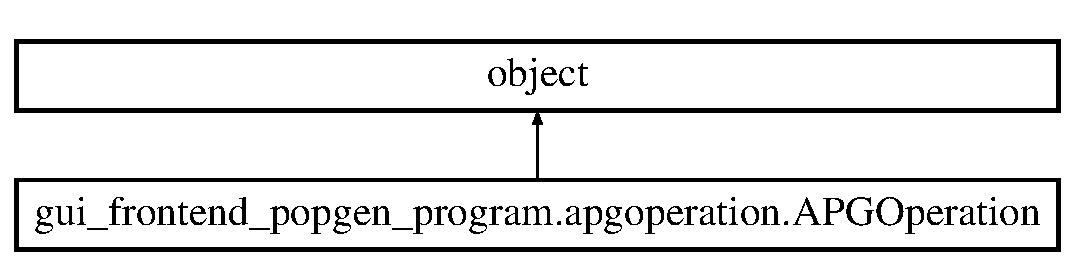
\includegraphics[height=2.000000cm]{classgui__frontend__popgen__program_1_1apgoperation_1_1APGOperation}
\end{center}
\end{figure}
\subsection*{Public Member Functions}
\begin{DoxyCompactItemize}
\item 
def {\bfseries \+\_\+\+\_\+init\+\_\+\+\_\+} (self)\hypertarget{classgui__frontend__popgen__program_1_1apgoperation_1_1APGOperation_afc397db8adcc2bec4674da7262e8a396}{}\label{classgui__frontend__popgen__program_1_1apgoperation_1_1APGOperation_afc397db8adcc2bec4674da7262e8a396}

\item 
def {\bfseries prepare\+Op} (self)\hypertarget{classgui__frontend__popgen__program_1_1apgoperation_1_1APGOperation_a180f6baaeaee3b461472180b7449a561}{}\label{classgui__frontend__popgen__program_1_1apgoperation_1_1APGOperation_a180f6baaeaee3b461472180b7449a561}

\item 
def {\bfseries do\+Op} (self)\hypertarget{classgui__frontend__popgen__program_1_1apgoperation_1_1APGOperation_ab6bbfcbcbbac6a9d98c5e768027d1645}{}\label{classgui__frontend__popgen__program_1_1apgoperation_1_1APGOperation_ab6bbfcbcbbac6a9d98c5e768027d1645}

\item 
def {\bfseries deliver\+Results} (self)\hypertarget{classgui__frontend__popgen__program_1_1apgoperation_1_1APGOperation_a847c2124b43acad2507ecc8807484e4d}{}\label{classgui__frontend__popgen__program_1_1apgoperation_1_1APGOperation_a847c2124b43acad2507ecc8807484e4d}

\end{DoxyCompactItemize}


\subsection{Detailed Description}
\begin{DoxyVerb}Abstract class PGOperation is to be implemented by subclasses.
Wraps the code required to perform a pop gen analysis, such as a simuPop simulation,
Or an Ne calculation.  Instantiated subclass objects are the expected type members 
of the PGGuiApp class objects attribute "gp_operation".
\end{DoxyVerb}
 

Definition at line 15 of file apgoperation.\+py.



The documentation for this class was generated from the following file\+:\begin{DoxyCompactItemize}
\item 
apgoperation.\+py\end{DoxyCompactItemize}

\hypertarget{classgui__frontend__popgen__program_1_1pgguiapp_1_1PGGuiApp}{}\section{gui\+\_\+frontend\+\_\+popgen\+\_\+program.\+pgguiapp.\+P\+G\+Gui\+App Class Reference}
\label{classgui__frontend__popgen__program_1_1pgguiapp_1_1PGGuiApp}\index{gui\+\_\+frontend\+\_\+popgen\+\_\+program.\+pgguiapp.\+P\+G\+Gui\+App@{gui\+\_\+frontend\+\_\+popgen\+\_\+program.\+pgguiapp.\+P\+G\+Gui\+App}}
Inheritance diagram for gui\+\_\+frontend\+\_\+popgen\+\_\+program.\+pgguiapp.\+P\+G\+Gui\+App\+:\begin{figure}[H]
\begin{center}
\leavevmode
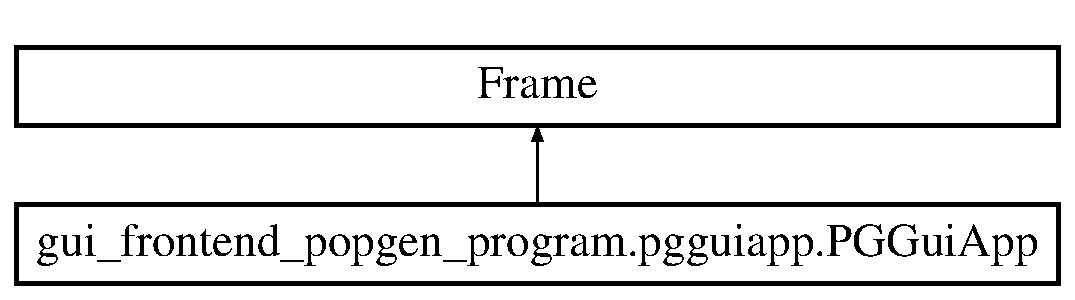
\includegraphics[height=2.000000cm]{classgui__frontend__popgen__program_1_1pgguiapp_1_1PGGuiApp}
\end{center}
\end{figure}
\subsection*{Public Member Functions}
\begin{DoxyCompactItemize}
\item 
def {\bfseries \+\_\+\+\_\+init\+\_\+\+\_\+} (self, master=None, o\+\_\+pg\+\_\+operation=None)\hypertarget{classgui__frontend__popgen__program_1_1pgguiapp_1_1PGGuiApp_add38f2accca7063b372c21581b98eb02}{}\label{classgui__frontend__popgen__program_1_1pgguiapp_1_1PGGuiApp_add38f2accca7063b372c21581b98eb02}

\item 
def \hyperlink{classgui__frontend__popgen__program_1_1pgguiapp_1_1PGGuiApp_af8c1f5a2a4cc57df73ea55266b000381}{op} (self)
\item 
def {\bfseries op} (self, o\+\_\+op)\hypertarget{classgui__frontend__popgen__program_1_1pgguiapp_1_1PGGuiApp_a8e20d8a2c9cc8b65c03250d5d64d6c75}{}\label{classgui__frontend__popgen__program_1_1pgguiapp_1_1PGGuiApp_a8e20d8a2c9cc8b65c03250d5d64d6c75}

\item 
def {\bfseries op} (self)\hypertarget{classgui__frontend__popgen__program_1_1pgguiapp_1_1PGGuiApp_af8c1f5a2a4cc57df73ea55266b000381}{}\label{classgui__frontend__popgen__program_1_1pgguiapp_1_1PGGuiApp_af8c1f5a2a4cc57df73ea55266b000381}

\end{DoxyCompactItemize}


\subsection{Detailed Description}
\begin{DoxyVerb}The standard way to deploy tkinter with application object that inherits Frame
(see example at https://docs.python.org/2/library/tkinter.html#Tkinter.Tk)
this app instantiated by driver code like, 

root = Tk()
app = Application(master=root)
app.mainloop()
root.destroy()
\end{DoxyVerb}
 

Definition at line 12 of file pgguiapp.\+py.



\subsection{Member Function Documentation}
\index{gui\+\_\+frontend\+\_\+popgen\+\_\+program\+::pgguiapp\+::\+P\+G\+Gui\+App@{gui\+\_\+frontend\+\_\+popgen\+\_\+program\+::pgguiapp\+::\+P\+G\+Gui\+App}!op@{op}}
\index{op@{op}!gui\+\_\+frontend\+\_\+popgen\+\_\+program\+::pgguiapp\+::\+P\+G\+Gui\+App@{gui\+\_\+frontend\+\_\+popgen\+\_\+program\+::pgguiapp\+::\+P\+G\+Gui\+App}}
\subsubsection[{\texorpdfstring{op(self)}{op(self)}}]{\setlength{\rightskip}{0pt plus 5cm}def gui\+\_\+frontend\+\_\+popgen\+\_\+program.\+pgguiapp.\+P\+G\+Gui\+App.\+op (
\begin{DoxyParamCaption}
\item[{}]{self}
\end{DoxyParamCaption}
)}\hypertarget{classgui__frontend__popgen__program_1_1pgguiapp_1_1PGGuiApp_af8c1f5a2a4cc57df73ea55266b000381}{}\label{classgui__frontend__popgen__program_1_1pgguiapp_1_1PGGuiApp_af8c1f5a2a4cc57df73ea55266b000381}
\begin{DoxyVerb}object that performs a pop gen operation by implementing abstract class PGOperation\end{DoxyVerb}
 

Definition at line 38 of file pgguiapp.\+py.


\begin{DoxyCode}
38     \textcolor{keyword}{def }\hyperlink{classgui__frontend__popgen__program_1_1pgguiapp_1_1PGGuiApp_af8c1f5a2a4cc57df73ea55266b000381}{op}( self ):
39         \textcolor{stringliteral}{"""object that performs a pop gen operation by implementing abstract class PGOperation"""}
40         \textcolor{keywordflow}{return} self.\hyperlink{classgui__frontend__popgen__program_1_1pgguiapp_1_1PGGuiApp_a3f3160336b7e4783d95734bc7835e7c7}{\_\_op}
\end{DoxyCode}


The documentation for this class was generated from the following file\+:\begin{DoxyCompactItemize}
\item 
pgguiapp.\+py\end{DoxyCompactItemize}

\hypertarget{classgui__frontend__popgen__program_1_1pgguisimupop_1_1PGGuiSimuPop}{}\section{gui\+\_\+frontend\+\_\+popgen\+\_\+program.\+pgguisimupop.\+P\+G\+Gui\+Simu\+Pop Class Reference}
\label{classgui__frontend__popgen__program_1_1pgguisimupop_1_1PGGuiSimuPop}\index{gui\+\_\+frontend\+\_\+popgen\+\_\+program.\+pgguisimupop.\+P\+G\+Gui\+Simu\+Pop@{gui\+\_\+frontend\+\_\+popgen\+\_\+program.\+pgguisimupop.\+P\+G\+Gui\+Simu\+Pop}}
Inheritance diagram for gui\+\_\+frontend\+\_\+popgen\+\_\+program.\+pgguisimupop.\+P\+G\+Gui\+Simu\+Pop\+:\begin{figure}[H]
\begin{center}
\leavevmode
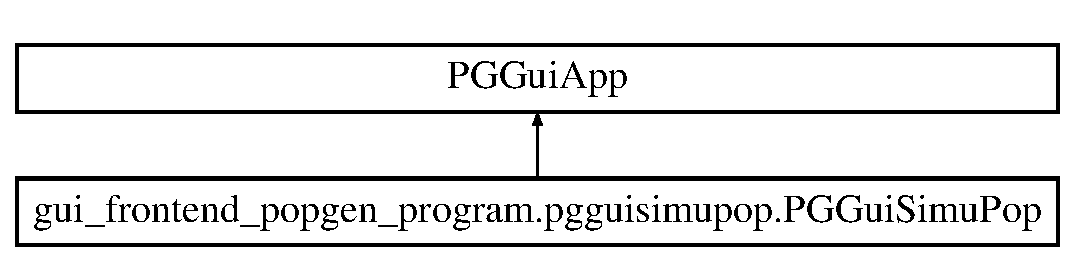
\includegraphics[height=2.000000cm]{classgui__frontend__popgen__program_1_1pgguisimupop_1_1PGGuiSimuPop}
\end{center}
\end{figure}
\subsection*{Public Member Functions}
\begin{DoxyCompactItemize}
\item 
def \hyperlink{classgui__frontend__popgen__program_1_1pgguisimupop_1_1PGGuiSimuPop_ae07df9c15703aef165688e29ace1c6ac}{\+\_\+\+\_\+init\+\_\+\+\_\+} (self, o\+\_\+parent, o\+\_\+simupop\+\_\+operation)
\end{DoxyCompactItemize}


\subsection{Detailed Description}
\begin{DoxyVerb}Subclass of PGGuiApp builds a gui and uses its member object "op", which
implements PGOperaion to enable a  simuPop simulation.
\end{DoxyVerb}
 

Definition at line 11 of file pgguisimupop.\+py.



\subsection{Constructor \& Destructor Documentation}
\index{gui\+\_\+frontend\+\_\+popgen\+\_\+program\+::pgguisimupop\+::\+P\+G\+Gui\+Simu\+Pop@{gui\+\_\+frontend\+\_\+popgen\+\_\+program\+::pgguisimupop\+::\+P\+G\+Gui\+Simu\+Pop}!\+\_\+\+\_\+init\+\_\+\+\_\+@{\+\_\+\+\_\+init\+\_\+\+\_\+}}
\index{\+\_\+\+\_\+init\+\_\+\+\_\+@{\+\_\+\+\_\+init\+\_\+\+\_\+}!gui\+\_\+frontend\+\_\+popgen\+\_\+program\+::pgguisimupop\+::\+P\+G\+Gui\+Simu\+Pop@{gui\+\_\+frontend\+\_\+popgen\+\_\+program\+::pgguisimupop\+::\+P\+G\+Gui\+Simu\+Pop}}
\subsubsection[{\texorpdfstring{\+\_\+\+\_\+init\+\_\+\+\_\+(self, o\+\_\+parent, o\+\_\+simupop\+\_\+operation)}{__init__(self, o_parent, o_simupop_operation)}}]{\setlength{\rightskip}{0pt plus 5cm}def gui\+\_\+frontend\+\_\+popgen\+\_\+program.\+pgguisimupop.\+P\+G\+Gui\+Simu\+Pop.\+\_\+\+\_\+init\+\_\+\+\_\+ (
\begin{DoxyParamCaption}
\item[{}]{self, }
\item[{}]{o\+\_\+parent, }
\item[{}]{o\+\_\+simupop\+\_\+operation}
\end{DoxyParamCaption}
)}\hypertarget{classgui__frontend__popgen__program_1_1pgguisimupop_1_1PGGuiSimuPop_ae07df9c15703aef165688e29ace1c6ac}{}\label{classgui__frontend__popgen__program_1_1pgguisimupop_1_1PGGuiSimuPop_ae07df9c15703aef165688e29ace1c6ac}
\begin{DoxyVerb}param o_parent is the Tk() Frame object on which the 
main window is based
param o_simupop_operation is the object that the widgets
control to setup and perform a simuPop simulation
\end{DoxyVerb}
 

Definition at line 16 of file pgguisimupop.\+py.


\begin{DoxyCode}
16     \textcolor{keyword}{def }\hyperlink{classgui__frontend__popgen__program_1_1pgguisimupop_1_1PGGuiSimuPop_ae07df9c15703aef165688e29ace1c6ac}{\_\_init\_\_}( self, o\_parent, o\_simupop\_operation ):
17         \textcolor{stringliteral}{'''}
18 \textcolor{stringliteral}{        param o\_parent is the Tk() Frame object on which the }
19 \textcolor{stringliteral}{        main window is based}
20 \textcolor{stringliteral}{        param o\_simupop\_operation is the object that the widgets}
21 \textcolor{stringliteral}{        control to setup and perform a simuPop simulation}
22 \textcolor{stringliteral}{        '''}
23         super().\hyperlink{classgui__frontend__popgen__program_1_1pgguisimupop_1_1PGGuiSimuPop_ae07df9c15703aef165688e29ace1c6ac}{\_\_init\_\_}( o\_parent, o\_simupop\_operation )
24 
\end{DoxyCode}


The documentation for this class was generated from the following file\+:\begin{DoxyCompactItemize}
\item 
pgguisimupop.\+py\end{DoxyCompactItemize}

\hypertarget{classgui__frontend__popgen__program_1_1pginputsimupop_1_1PGInputSimuPop}{}\section{gui\+\_\+frontend\+\_\+popgen\+\_\+program.\+pginputsimupop.\+P\+G\+Input\+Simu\+Pop Class Reference}
\label{classgui__frontend__popgen__program_1_1pginputsimupop_1_1PGInputSimuPop}\index{gui\+\_\+frontend\+\_\+popgen\+\_\+program.\+pginputsimupop.\+P\+G\+Input\+Simu\+Pop@{gui\+\_\+frontend\+\_\+popgen\+\_\+program.\+pginputsimupop.\+P\+G\+Input\+Simu\+Pop}}
Inheritance diagram for gui\+\_\+frontend\+\_\+popgen\+\_\+program.\+pginputsimupop.\+P\+G\+Input\+Simu\+Pop\+:\begin{figure}[H]
\begin{center}
\leavevmode
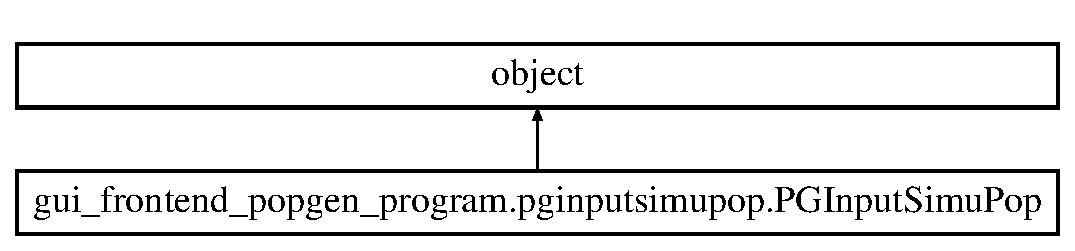
\includegraphics[height=2.000000cm]{classgui__frontend__popgen__program_1_1pginputsimupop_1_1PGInputSimuPop}
\end{center}
\end{figure}
\subsection*{Public Member Functions}
\begin{DoxyCompactItemize}
\item 
def {\bfseries \+\_\+\+\_\+init\+\_\+\+\_\+} (self, s\+\_\+config\+\_\+file=None, s\+\_\+resources\+\_\+file=None)\hypertarget{classgui__frontend__popgen__program_1_1pginputsimupop_1_1PGInputSimuPop_a64b16863b0a6048d9451ec8b64e3a79f}{}\label{classgui__frontend__popgen__program_1_1pginputsimupop_1_1PGInputSimuPop_a64b16863b0a6048d9451ec8b64e3a79f}

\end{DoxyCompactItemize}


\subsection{Detailed Description}
\begin{DoxyVerb}Object meant to fetch parameter values and prepare them for 
use in a simuPop simulation.  

Object to be passed to a PGOpSimuPop object, which is, in turn,
passed to a PGGuiSimuPop object, so that the widgets can then access
defs in this input object, in order to, for example, show or allow
changes in parameter values for users before they run the simulation.
\end{DoxyVerb}
 

Definition at line 11 of file pginputsimupop.\+py.



The documentation for this class was generated from the following file\+:\begin{DoxyCompactItemize}
\item 
pginputsimupop.\+py\end{DoxyCompactItemize}

\hypertarget{classgui__frontend__popgen__program_1_1pgmenubuilder_1_1PGMenuBuilder}{}\section{gui\+\_\+frontend\+\_\+popgen\+\_\+program.\+pgmenubuilder.\+P\+G\+Menu\+Builder Class Reference}
\label{classgui__frontend__popgen__program_1_1pgmenubuilder_1_1PGMenuBuilder}\index{gui\+\_\+frontend\+\_\+popgen\+\_\+program.\+pgmenubuilder.\+P\+G\+Menu\+Builder@{gui\+\_\+frontend\+\_\+popgen\+\_\+program.\+pgmenubuilder.\+P\+G\+Menu\+Builder}}
Inheritance diagram for gui\+\_\+frontend\+\_\+popgen\+\_\+program.\+pgmenubuilder.\+P\+G\+Menu\+Builder\+:\begin{figure}[H]
\begin{center}
\leavevmode
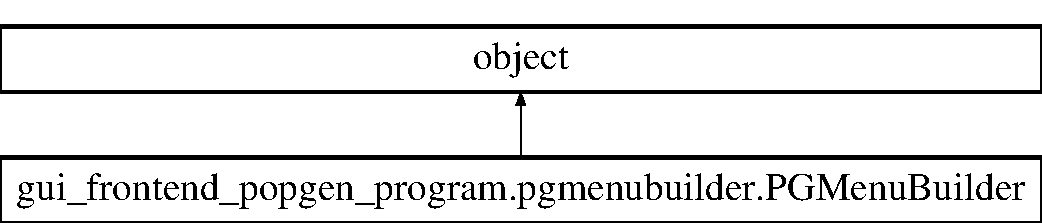
\includegraphics[height=2.000000cm]{classgui__frontend__popgen__program_1_1pgmenubuilder_1_1PGMenuBuilder}
\end{center}
\end{figure}
\subsection*{Public Member Functions}
\begin{DoxyCompactItemize}
\item 
def \hyperlink{classgui__frontend__popgen__program_1_1pgmenubuilder_1_1PGMenuBuilder_a09e525c5459e1d60f7aaa31cc7b6e0ea}{\+\_\+\+\_\+init\+\_\+\+\_\+} (self, s\+\_\+config\+\_\+file, o\+\_\+parent, o\+\_\+pg\+\_\+operation, i\+\_\+tearoff=0)
\item 
def \hyperlink{classgui__frontend__popgen__program_1_1pgmenubuilder_1_1PGMenuBuilder_a717ed3e9feead39c81f11bf47a2d0cf4}{get\+\_\+add\+\_\+command\+\_\+params\+\_\+and\+\_\+args} (self, o\+\_\+config, s\+\_\+menu\+\_\+label)
\item 
def \hyperlink{classgui__frontend__popgen__program_1_1pgmenubuilder_1_1PGMenuBuilder_a74a9d002649b744dbc442a53a16dbc29}{menu} (self)
\item 
def {\bfseries menu} (self, i\+\_\+value)\hypertarget{classgui__frontend__popgen__program_1_1pgmenubuilder_1_1PGMenuBuilder_a02e8c4624d6ed366a5c8c942b8fcf609}{}\label{classgui__frontend__popgen__program_1_1pgmenubuilder_1_1PGMenuBuilder_a02e8c4624d6ed366a5c8c942b8fcf609}

\item 
def {\bfseries menu} (self)\hypertarget{classgui__frontend__popgen__program_1_1pgmenubuilder_1_1PGMenuBuilder_a74a9d002649b744dbc442a53a16dbc29}{}\label{classgui__frontend__popgen__program_1_1pgmenubuilder_1_1PGMenuBuilder_a74a9d002649b744dbc442a53a16dbc29}

\end{DoxyCompactItemize}
\subsection*{Static Public Attributes}
\begin{DoxyCompactItemize}
\item 
list {\bfseries C\+O\+N\+F\+I\+G\+\_\+\+O\+P\+T\+I\+O\+N\+S\+\_\+\+N\+O\+N\+\_\+\+C\+O\+M\+M\+A\+N\+D\+\_\+\+A\+R\+GS} = \mbox{[} \char`\"{}parent\char`\"{}, \char`\"{}menu\+\_\+underline\char`\"{} \mbox{]}\hypertarget{classgui__frontend__popgen__program_1_1pgmenubuilder_1_1PGMenuBuilder_abebcbf4c07d8e8dbf43675e314088d5a}{}\label{classgui__frontend__popgen__program_1_1pgmenubuilder_1_1PGMenuBuilder_abebcbf4c07d8e8dbf43675e314088d5a}

\item 
{\bfseries o\+\_\+this\+\_\+menu} = Menu( self.\+\_\+\+\_\+menubar, tearoff = self.\+\_\+\+\_\+tearoff )\hypertarget{classgui__frontend__popgen__program_1_1pgmenubuilder_1_1PGMenuBuilder_abeb76d0bd440b112327fac69f10b5935}{}\label{classgui__frontend__popgen__program_1_1pgmenubuilder_1_1PGMenuBuilder_abeb76d0bd440b112327fac69f10b5935}

\item 
{\bfseries ld\+\_\+args} = self.\+get\+\_\+add\+\_\+command\+\_\+params\+\_\+and\+\_\+args( o\+\_\+config, s\+\_\+menu\+\_\+label )\hypertarget{classgui__frontend__popgen__program_1_1pgmenubuilder_1_1PGMenuBuilder_aea1757aeb44b06f9c0af5dbcb96e11f1}{}\label{classgui__frontend__popgen__program_1_1pgmenubuilder_1_1PGMenuBuilder_aea1757aeb44b06f9c0af5dbcb96e11f1}

\item 
{\bfseries dv\+\_\+menu\+\_\+values} = self.\+\_\+\+\_\+get\+\_\+menu\+\_\+values( o\+\_\+config, s\+\_\+menu\+\_\+label )\hypertarget{classgui__frontend__popgen__program_1_1pgmenubuilder_1_1PGMenuBuilder_af9a14f67b0e3ba344be2dd782dfa4b3a}{}\label{classgui__frontend__popgen__program_1_1pgmenubuilder_1_1PGMenuBuilder_af9a14f67b0e3ba344be2dd782dfa4b3a}

\item 
{\bfseries label}\hypertarget{classgui__frontend__popgen__program_1_1pgmenubuilder_1_1PGMenuBuilder_ae1be7da55a8c3709b2490344e1d393a3}{}\label{classgui__frontend__popgen__program_1_1pgmenubuilder_1_1PGMenuBuilder_ae1be7da55a8c3709b2490344e1d393a3}

\item 
{\bfseries menu}\hypertarget{classgui__frontend__popgen__program_1_1pgmenubuilder_1_1PGMenuBuilder_ab4e38859621f23a5abb5bebf2f51e466}{}\label{classgui__frontend__popgen__program_1_1pgmenubuilder_1_1PGMenuBuilder_ab4e38859621f23a5abb5bebf2f51e466}

\item 
{\bfseries underline}\hypertarget{classgui__frontend__popgen__program_1_1pgmenubuilder_1_1PGMenuBuilder_a860a087d041bb103ea6c73b93905e142}{}\label{classgui__frontend__popgen__program_1_1pgmenubuilder_1_1PGMenuBuilder_a860a087d041bb103ea6c73b93905e142}

\end{DoxyCompactItemize}


\subsection{Detailed Description}
\begin{DoxyVerb}Instantiates a tkinter menu_bar, with parent gui object (usually the main window) 
as given by __init__ param, and populates it by reading a list of menu items and 
parameters from a configuration file, also an __init__ param. The menus get their 
command callback defs, as named in the configuration file, in the class object 
passed as init param o_pg_operation.

The configuration file key=value entries inside each [section] are of two classes:

1. keys that are not param keywords for the call to menu.add_command.  These include 
    (a) "parent=value", which tells the
    builder which of the file labels (sections in the config file) is the parent menu
    to it's submenu.  As of 20160116 this is not implemented, and only parent=None (unquoted) 
    is allowed.
    (b) "menu_underline=value", where value is an (zero-based) index into the menu label name 
    (as given by the section name).

2. key=value pairs whose keys are param keywords (like "accelerator").  Keys must match exactly
    prarm names in the menu.add_command definition's param list.  Their values should be 
    entered in square brackets like a python list, with one entry for each of the menu items.  
    If the nth item is to be "seperator" item, the nth item in the label list should be 
    "sep", and other items like "command" or accelerator, can be any value (ex: None), 
    as they will be ignored.

For example, a menubar with 2 items "File" and "Edit", each with 2 menu items, with
Edit having a seperator between its items would look like this: 

#file menu
[File]
parent=None
#which characters to underline in the File label:
menu_underline=0
label=[ "New" , "Open" ]
#which characters to underline in the menu items:
underline=[ 0, 0 ]
accelerator=[ "Ctrl+N","Ctrl+O" ]
command=[ "new_file", "open_file" ]

#edit menu
[Edit]
parent=None
menu_underline=0
label=["Undo","sep","Options"]
underline=[ 1,None, 1 ]
accelerator=["Ctrl+Z", None, "Ctrl+T"]
command=[ "undo", None, "showopts" ]  
\end{DoxyVerb}
 

Definition at line 14 of file pgmenubuilder.\+py.



\subsection{Constructor \& Destructor Documentation}
\index{gui\+\_\+frontend\+\_\+popgen\+\_\+program\+::pgmenubuilder\+::\+P\+G\+Menu\+Builder@{gui\+\_\+frontend\+\_\+popgen\+\_\+program\+::pgmenubuilder\+::\+P\+G\+Menu\+Builder}!\+\_\+\+\_\+init\+\_\+\+\_\+@{\+\_\+\+\_\+init\+\_\+\+\_\+}}
\index{\+\_\+\+\_\+init\+\_\+\+\_\+@{\+\_\+\+\_\+init\+\_\+\+\_\+}!gui\+\_\+frontend\+\_\+popgen\+\_\+program\+::pgmenubuilder\+::\+P\+G\+Menu\+Builder@{gui\+\_\+frontend\+\_\+popgen\+\_\+program\+::pgmenubuilder\+::\+P\+G\+Menu\+Builder}}
\subsubsection[{\texorpdfstring{\+\_\+\+\_\+init\+\_\+\+\_\+(self, s\+\_\+config\+\_\+file, o\+\_\+parent, o\+\_\+pg\+\_\+operation, i\+\_\+tearoff=0)}{__init__(self, s_config_file, o_parent, o_pg_operation, i_tearoff=0)}}]{\setlength{\rightskip}{0pt plus 5cm}def gui\+\_\+frontend\+\_\+popgen\+\_\+program.\+pgmenubuilder.\+P\+G\+Menu\+Builder.\+\_\+\+\_\+init\+\_\+\+\_\+ (
\begin{DoxyParamCaption}
\item[{}]{self, }
\item[{}]{s\+\_\+config\+\_\+file, }
\item[{}]{o\+\_\+parent, }
\item[{}]{o\+\_\+pg\+\_\+operation, }
\item[{}]{i\+\_\+tearoff = {\ttfamily 0}}
\end{DoxyParamCaption}
)}\hypertarget{classgui__frontend__popgen__program_1_1pgmenubuilder_1_1PGMenuBuilder_a09e525c5459e1d60f7aaa31cc7b6e0ea}{}\label{classgui__frontend__popgen__program_1_1pgmenubuilder_1_1PGMenuBuilder_a09e525c5459e1d60f7aaa31cc7b6e0ea}
\begin{DoxyVerb}param s_config_file gives menu attribute values (see module documentation)
param o_parent is the Tk widget parent of the menu this object builds
param o_pg_operation is a class object that has the definitions
that match the command names to be bound to the menus ('command' 
option values in the config file)
param i_tearoff tells the gui whether the menu items can be dragged off of 
    the parent menubar (tearoff=1) or not (tearoff=0)
\end{DoxyVerb}
 

Definition at line 65 of file pgmenubuilder.\+py.


\begin{DoxyCode}
65     \textcolor{keyword}{def }\hyperlink{classgui__frontend__popgen__program_1_1pgmenubuilder_1_1PGMenuBuilder_a09e525c5459e1d60f7aaa31cc7b6e0ea}{\_\_init\_\_}( self, s\_config\_file, o\_parent, o\_pg\_operation, i\_tearoff=0 ):
66         \textcolor{stringliteral}{'''}
67 \textcolor{stringliteral}{        param s\_config\_file gives menu attribute values (see module documentation)}
68 \textcolor{stringliteral}{        param o\_parent is the Tk widget parent of the menu this object builds}
69 \textcolor{stringliteral}{        param o\_pg\_operation is a class object that has the definitions}
70 \textcolor{stringliteral}{                that match the command names to be bound to the menus ('command' }
71 \textcolor{stringliteral}{                option values in the config file)}
72 \textcolor{stringliteral}{        param i\_tearoff tells the gui whether the menu items can be dragged off of }
73 \textcolor{stringliteral}{            the parent menubar (tearoff=1) or not (tearoff=0)}
74 \textcolor{stringliteral}{        '''}
75 
76         self.\_\_menubar = \textcolor{keywordtype}{None}
77         self.\_\_pg\_operation = o\_pg\_operation
78         self.\_\_tearoff = i\_tearoff
79         self.\_\_parent=o\_parent
80         o\_config = self.\_\_get\_menu\_info( s\_config\_file )
81         self.\_\_build\_menu( o\_config )
82         \textcolor{keywordflow}{return}
\end{DoxyCode}


\subsection{Member Function Documentation}
\index{gui\+\_\+frontend\+\_\+popgen\+\_\+program\+::pgmenubuilder\+::\+P\+G\+Menu\+Builder@{gui\+\_\+frontend\+\_\+popgen\+\_\+program\+::pgmenubuilder\+::\+P\+G\+Menu\+Builder}!get\+\_\+add\+\_\+command\+\_\+params\+\_\+and\+\_\+args@{get\+\_\+add\+\_\+command\+\_\+params\+\_\+and\+\_\+args}}
\index{get\+\_\+add\+\_\+command\+\_\+params\+\_\+and\+\_\+args@{get\+\_\+add\+\_\+command\+\_\+params\+\_\+and\+\_\+args}!gui\+\_\+frontend\+\_\+popgen\+\_\+program\+::pgmenubuilder\+::\+P\+G\+Menu\+Builder@{gui\+\_\+frontend\+\_\+popgen\+\_\+program\+::pgmenubuilder\+::\+P\+G\+Menu\+Builder}}
\subsubsection[{\texorpdfstring{get\+\_\+add\+\_\+command\+\_\+params\+\_\+and\+\_\+args(self, o\+\_\+config, s\+\_\+menu\+\_\+label)}{get_add_command_params_and_args(self, o_config, s_menu_label)}}]{\setlength{\rightskip}{0pt plus 5cm}def gui\+\_\+frontend\+\_\+popgen\+\_\+program.\+pgmenubuilder.\+P\+G\+Menu\+Builder.\+get\+\_\+add\+\_\+command\+\_\+params\+\_\+and\+\_\+args (
\begin{DoxyParamCaption}
\item[{}]{self, }
\item[{}]{o\+\_\+config, }
\item[{}]{s\+\_\+menu\+\_\+label}
\end{DoxyParamCaption}
)}\hypertarget{classgui__frontend__popgen__program_1_1pgmenubuilder_1_1PGMenuBuilder_a717ed3e9feead39c81f11bf47a2d0cf4}{}\label{classgui__frontend__popgen__program_1_1pgmenubuilder_1_1PGMenuBuilder_a717ed3e9feead39c81f11bf47a2d0cf4}
\begin{DoxyVerb}returns a list of dictionaries, one for each menu item, of the param=value
settings for calls to menu.add_command.  We skip the config key=value for keys
that are not part of the params needed for add_command. 
\end{DoxyVerb}
 

Definition at line 115 of file pgmenubuilder.\+py.


\begin{DoxyCode}
115     \textcolor{keyword}{def }\hyperlink{classgui__frontend__popgen__program_1_1pgmenubuilder_1_1PGMenuBuilder_a717ed3e9feead39c81f11bf47a2d0cf4}{get\_add\_command\_params\_and\_args}( self,  o\_config, s\_menu\_label ):
116         \textcolor{stringliteral}{'''}
117 \textcolor{stringliteral}{        returns a list of dictionaries, one for each menu item, of the param=value}
118 \textcolor{stringliteral}{        settings for calls to menu.add\_command.  We skip the config key=value for keys}
119 \textcolor{stringliteral}{        that are not part of the params needed for add\_command. }
120 \textcolor{stringliteral}{        '''}
121 
122         l\_keyword\_menu\_params = o\_config.options( s\_menu\_label )    
123 
124         \textcolor{comment}{#how many items on this menu should equal number of labels:}
125         i\_num\_items = self.\hyperlink{classgui__frontend__popgen__program_1_1pgmenubuilder_1_1PGMenuBuilder_a40e63e390562a2a3eecacef8a72ddbef}{\_\_get\_num\_labels\_menu}( o\_config, s\_menu\_label )
126 
127         ld\_args = [ \{\} \textcolor{keywordflow}{for} idx \textcolor{keywordflow}{in} range( i\_num\_items ) ]
128 
129         \textcolor{comment}{#for each submenu item, we get a dict of keyword:value to pass to "add\_command"}
130         \textcolor{keywordflow}{for} s\_keyword \textcolor{keywordflow}{in} l\_keyword\_menu\_params:
131             s\_vals=o\_config.get( s\_menu\_label, s\_keyword )
132 
133             \textcolor{comment}{#for each keyword that is a param name in the menu.add\_command call}
134             \textcolor{keywordflow}{if} s\_keyword \textcolor{keywordflow}{not} \textcolor{keywordflow}{in} PGMenuBuilder.CONFIG\_OPTIONS\_NON\_COMMAND\_ARGS:
135 
136                 l\_vals=eval( s\_vals )
137 
138                 \textcolor{keywordflow}{if} len( l\_vals ) != i\_num\_items:
139                     \textcolor{keywordflow}{raise} Exception( \textcolor{stringliteral}{"in pgmenubuilder, config entry should have "} \(\backslash\)
140                             + \textcolor{stringliteral}{"one item for each label, but the option with keyname, "} \(\backslash\)
141                             + s\_keyword + \textcolor{stringliteral}{"does not."} )
142                 \textcolor{comment}{#end if wrong number values}
143                 
144                 \textcolor{comment}{#if this is the list of command values (callback defs) }
145                 \textcolor{comment}{#for each submenu item,}
146                 \textcolor{comment}{#then we must be able to find it among the attributes}
147                 \textcolor{comment}{#of our member operation object}
148                 \textcolor{comment}{#note: if "sep" is the label, we set other param values }
149                 \textcolor{comment}{#to None, but they are ignored (see for loop below)}
150                 \textcolor{keywordflow}{if} s\_keyword ==\textcolor{stringliteral}{"command"}:
151                     l\_vals = [ getattr( self.\hyperlink{classgui__frontend__popgen__program_1_1pgmenubuilder_1_1PGMenuBuilder_a551e6b6a9f0b2e46f543d36dfc8af0fb}{\_\_pg\_operation}, thisval ) \(\backslash\)
152                             \textcolor{keywordflow}{if} thisval \textcolor{keywordflow}{is} \textcolor{keywordflow}{not} \textcolor{keywordtype}{None} \(\backslash\)
153                             \textcolor{keywordflow}{else} \textcolor{keywordtype}{None} \textcolor{keywordflow}{for} thisval \textcolor{keywordflow}{in} l\_vals ]
154                 \textcolor{comment}{#end if command list}
155 
156                 \textcolor{keywordflow}{for} idx \textcolor{keywordflow}{in} range( i\_num\_items ):
157                     ld\_args[ idx ][ s\_keyword ] = l\_vals[ idx ]
158                 \textcolor{comment}{#end for each item}
159             \textcolor{comment}{#end if not a param keyword for add\_command}
160         \textcolor{comment}{#end for each keyword}
161         \textcolor{keywordflow}{return} ld\_args
\end{DoxyCode}
\index{gui\+\_\+frontend\+\_\+popgen\+\_\+program\+::pgmenubuilder\+::\+P\+G\+Menu\+Builder@{gui\+\_\+frontend\+\_\+popgen\+\_\+program\+::pgmenubuilder\+::\+P\+G\+Menu\+Builder}!menu@{menu}}
\index{menu@{menu}!gui\+\_\+frontend\+\_\+popgen\+\_\+program\+::pgmenubuilder\+::\+P\+G\+Menu\+Builder@{gui\+\_\+frontend\+\_\+popgen\+\_\+program\+::pgmenubuilder\+::\+P\+G\+Menu\+Builder}}
\subsubsection[{\texorpdfstring{menu(self)}{menu(self)}}]{\setlength{\rightskip}{0pt plus 5cm}def gui\+\_\+frontend\+\_\+popgen\+\_\+program.\+pgmenubuilder.\+P\+G\+Menu\+Builder.\+menu (
\begin{DoxyParamCaption}
\item[{}]{self}
\end{DoxyParamCaption}
)}\hypertarget{classgui__frontend__popgen__program_1_1pgmenubuilder_1_1PGMenuBuilder_a74a9d002649b744dbc442a53a16dbc29}{}\label{classgui__frontend__popgen__program_1_1pgmenubuilder_1_1PGMenuBuilder_a74a9d002649b744dbc442a53a16dbc29}
\begin{DoxyVerb}menu, tk.TKMenu object\end{DoxyVerb}
 

Definition at line 208 of file pgmenubuilder.\+py.


\begin{DoxyCode}
208     \textcolor{keyword}{def }menu(self):
209         \textcolor{stringliteral}{"""menu, tk.TKMenu object"""}
210         \textcolor{keywordflow}{return} self.\hyperlink{classgui__frontend__popgen__program_1_1pgmenubuilder_1_1PGMenuBuilder_abc2334fcb2c9693bd6aae7f8fde48db9}{\_\_menubar}
\end{DoxyCode}


The documentation for this class was generated from the following file\+:\begin{DoxyCompactItemize}
\item 
pgmenubuilder.\+py\end{DoxyCompactItemize}

\hypertarget{classgui__frontend__popgen__program_1_1pgopsimupop_1_1PGOpSimuPop}{}\section{gui\+\_\+frontend\+\_\+popgen\+\_\+program.\+pgopsimupop.\+P\+G\+Op\+Simu\+Pop Class Reference}
\label{classgui__frontend__popgen__program_1_1pgopsimupop_1_1PGOpSimuPop}\index{gui\+\_\+frontend\+\_\+popgen\+\_\+program.\+pgopsimupop.\+P\+G\+Op\+Simu\+Pop@{gui\+\_\+frontend\+\_\+popgen\+\_\+program.\+pgopsimupop.\+P\+G\+Op\+Simu\+Pop}}
Inheritance diagram for gui\+\_\+frontend\+\_\+popgen\+\_\+program.\+pgopsimupop.\+P\+G\+Op\+Simu\+Pop\+:\begin{figure}[H]
\begin{center}
\leavevmode
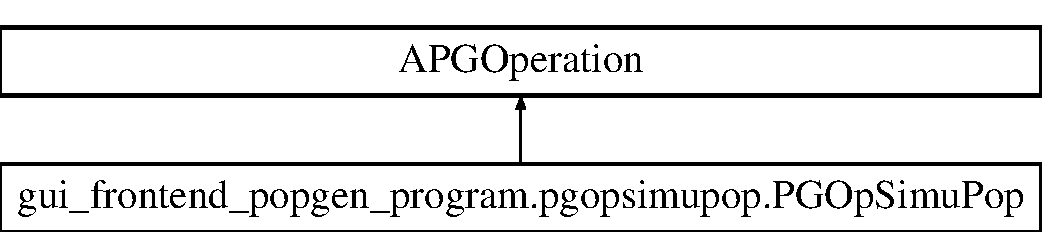
\includegraphics[height=2.000000cm]{classgui__frontend__popgen__program_1_1pgopsimupop_1_1PGOpSimuPop}
\end{center}
\end{figure}
\subsection*{Public Member Functions}
\begin{DoxyCompactItemize}
\item 
def {\bfseries \+\_\+\+\_\+init\+\_\+\+\_\+} (self, o\+\_\+input=None, o\+\_\+output=None)\hypertarget{classgui__frontend__popgen__program_1_1pgopsimupop_1_1PGOpSimuPop_a531e6d5be4c802ded5589b13ea608bfa}{}\label{classgui__frontend__popgen__program_1_1pgopsimupop_1_1PGOpSimuPop_a531e6d5be4c802ded5589b13ea608bfa}

\item 
def {\bfseries prepare\+Op} (self)\hypertarget{classgui__frontend__popgen__program_1_1pgopsimupop_1_1PGOpSimuPop_aef856baf7931e68c08afc1a5b193ef57}{}\label{classgui__frontend__popgen__program_1_1pgopsimupop_1_1PGOpSimuPop_aef856baf7931e68c08afc1a5b193ef57}

\item 
def {\bfseries do\+Op} (self)\hypertarget{classgui__frontend__popgen__program_1_1pgopsimupop_1_1PGOpSimuPop_a4a780914302b14c112b122279084678c}{}\label{classgui__frontend__popgen__program_1_1pgopsimupop_1_1PGOpSimuPop_a4a780914302b14c112b122279084678c}

\item 
def {\bfseries deliver\+Results} (self)\hypertarget{classgui__frontend__popgen__program_1_1pgopsimupop_1_1PGOpSimuPop_aec833df77985af0767c8a39c2c58f411}{}\label{classgui__frontend__popgen__program_1_1pgopsimupop_1_1PGOpSimuPop_aec833df77985af0767c8a39c2c58f411}

\end{DoxyCompactItemize}


\subsection{Detailed Description}
\begin{DoxyVerb}This class inherits its basic interface from class APGOperation, with its 3
basic defs "prepareOp", "doOP", and "deliverResults"

Its motivating role is to be a member object of a PGGuiApp object, and to contain the
defs that do a simupop simulation and give results back to the gui.

Should use no GUI classes, but strictly utils or pop-gen calls.

This object has member two objects, an input object that fetches and prepares the
data needed for the simuPop run, and an output object that formats and/or delivers
the results.   These objects are exposed to users via getters.  The defs in these 
member objects can thus be accessed by gui widgets when this class is PGOP object 
is instantiated and used as a member of a PGGuiApp object
\end{DoxyVerb}
 

Definition at line 11 of file pgopsimupop.\+py.



The documentation for this class was generated from the following file\+:\begin{DoxyCompactItemize}
\item 
pgopsimupop.\+py\end{DoxyCompactItemize}

%--- End generated contents ---

% Index
\backmatter
\newpage
\phantomsection
\clearemptydoublepage
\addcontentsline{toc}{chapter}{Index}
\printindex

\end{document}
